\documentclass{article}
\usepackage[margin=0.6in]{geometry}
\usepackage{amsmath}
\usepackage{amssymb}
\usepackage{graphicx}
\usepackage{float}
\usepackage{bookmark}

\title{Solutions to the Assignment - 3 : CS5560 - \\
Probabilistic Models in Machine Learning}
\author{Vishwak Srinivasan\\
\texttt{CS15BTECH11043}}
\date{}

\begin{document}
\maketitle

\section*{Mean function learned from the data}
The dataset had 18 attributes in total: 14 input and 4 output. Below is the functional form obtained:
\begin{multline}
f^{*}(\mathbf{x}) =
\begin{bmatrix}
217.6479 \\ 217.5795 \\ 217.5328 \\ 217.5277
\end{bmatrix}_{4 \times 1} + 
\begin{bmatrix} 
3.3299 & 3.0769 & 5.217 & -16.7299 & -16.3969 & 1.039 & 1.0495 \\
3.9587 & -1.5067 & -3.023 & -9.2756 & -0.0898 & 38.7406 & 47.3529 \\
\hline
3.3301 & 3.074 & 5.1879 & -16.6925 & -16.3586 & 1.0312 & 1.0438 \\
4.0167 & -1.5123 & -3.0284 & -9.293 & -0.0738 & 38.2147 & 47.1147 \\
\hline
3.3302 & 3.0749 & 5.1879 & -16.6937 & -16.3549 & 1.0331 & 1.045 \\
4.02 & -1.5073 & -3.026 & -9.2805 & -0.0805 & 38.176 & 47.1172 \\
\hline
3.3304 & 3.0743 & 5.1856 & -16.693 & -16.356 & 1.0321 & 1.0441 \\
4.0186 & -1.512 & -3.021 & -9.2795 & -0.0741 & 38.1949 & 47.1045
\end{bmatrix}_{4 \times 14} \\\left(\mathbf{x} -
\begin{bmatrix}
80.4154 \\ 80.4154 \\ 25.5131 \\ 13.9359 \\ 13.9359 \\ 17.3711 \\ 17.3711 \\5. \\ 2.4486
\\ 2.4486 \\ 0.5 \\ 0.5 \\ 0.5 \\ 0.5
\end{bmatrix}_{14 \times 1} \right)
\end{multline}

\section*{Mean Squared Loss over the entire dataset with the learned function for each output variable}
\begin{center}
\begin{tabular}{|c|c|}
\hline
Output Variable 1 & 302688.3187 \\ \hline Output Variable 2 & 302028.1803 \\
\hline
Output Variable 3 & 302036.0746 \\ \hline Output Variable 4 & 302042.7921 \\
\hline
\end{tabular}
\end{center}

\section*{Prototypes of functions}
First, I compute the mean of the datapoints in the dataset using \texttt{np.mean}. Then for every datapoint \(z = (x, y)\), I compute the centered outer product i.e., \(z - \hat{\mu}\), where \(\mu\) is the estimated mean - using \texttt{np.outer}. The average of these outer products would be the estimated covariance. After this, I parition the matrix into separate block matrices using \texttt{np.hsplit} and \texttt{np.vsplit}. Now I compute the function form using the simplication based on the Schur complement inverse. For matrix multiplication, I use \texttt{np.matmul}.

\section*{Output snapshot}
\begin{figure}[H]
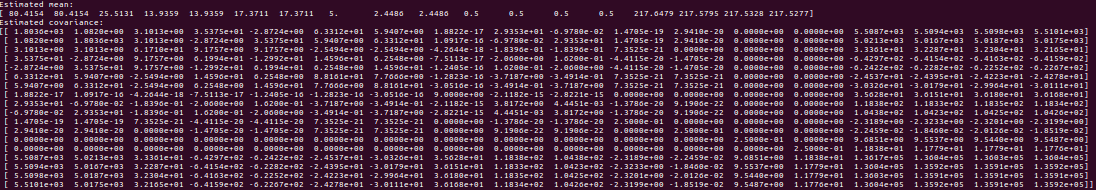
\includegraphics[width=0.95\textwidth]{./images/output-1.png}
\caption{Output after computing the estimated means and covariances}
\end{figure}

\begin{figure}[H]
\begin{minipage}{0.66\linewidth}
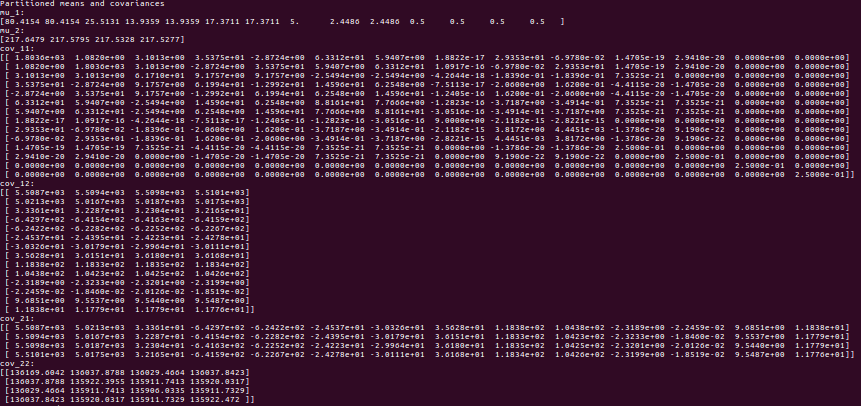
\includegraphics[width=0.95\textwidth]{./images/output-2.png}
\caption{Output after computing the partitioning the means and covariances}
\end{minipage}
\hfill
\begin{minipage}{0.30\linewidth}
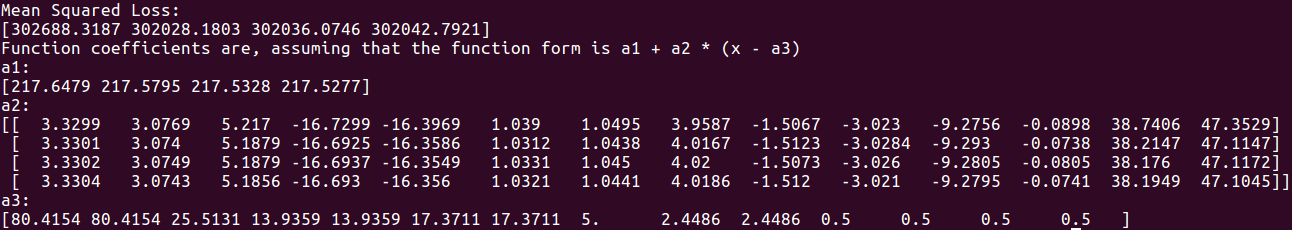
\includegraphics[width=0.95\textwidth]{./images/output-3.png}
\caption{Output after computing the mean function learned}
\end{minipage}
\end{figure}

\section*{Trying out some modifications on the dataset based on dataset description}
I made two changes to the dataset. For attributes 1-10 (inclusive), I considered the \(\log_{2}\) of the actual values, since the values of those attributes were powers of 2. For the output values, I considered the natural logarithm of the original values as suggested in the dataset description. With these modifications, I re-ran the code and obtained a function with a much better fit. The mean squared loss over the entire dataset with the learned function for each output variable is tabulated below:
\begin{center}
\begin{tabular}{|c|c|}
\hline
Output Variable 1 & 3.296 \\ \hline Output Variable 2 & 3.2896 \\
\hline
Output Variable 3 & 3.2934 \\ \hline Output Variable 4 & 3.2929 \\
\hline
\end{tabular}
\end{center}

\end{document}
